\documentclass{standalone}
\usepackage{tikz}
\usepackage{fontawesome}
\usetikzlibrary{arrows.meta, automata, calc, positioning, quotes, calc, shadings, shadows, shapes.arrows}

\begin{document}

    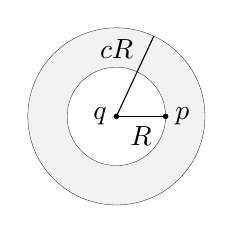
\begin{tikzpicture}
        
        \node[circle, ultra thin, draw, minimum size=2.25cm, fill=black!10, fill opacity=0.5] (X) at (0,0){};
        \node[circle, ultra thin, draw, minimum size=1.25cm, fill=white] (R) at (0,0){};

        \fill[radius=1pt](0,0) circle[] node[left] {$q$};
        \fill[radius=1pt](0.625,0) circle[] node[right] {$p$};
        % \fill[radius=1pt](0.5,0) circle[] node[left] {$p'$};
        \draw (0,0) -- node[below]{$R$} (0.625, 0);
        \draw (X.center) -- node[above left, yshift=0.1cm, xshift=0.1cm]{$cR$} (65:1.125);


    \end{tikzpicture}

\end{document}